\documentclass{jsarticle}
\usepackage{amsmath, smssymb, amsfonts}
\usepackage{newtxtext, newtxmath}
\usepackage{latexsym}
\usepackage{mathrsfs}
\usepackage{mathtools}
\usepackage{textcomp}
\usepackage{mathcomp}
\usepackage[dvipdfmx]{graphicx, xcolor}
\usepackage{float}
\usepackage{wrapfig}	% must be after float package.
\usepackage{subcaption}
\usepackage{booktabs}
\usepackage{url}
\usepackage{listings, jvlisting, color}

\definecolor{OliveGreen}{rgb}{0.0,0.6,0.0}
\definecolor{Orenge}{rgb}{0.89,0.55,0}
\definecolor{SkyBlue}{rgb}{0.28, 0.28, 0.95}
\lstset{
  language={C++}, % 言語の指定
  basicstyle={\ttfamily},
  identifierstyle={\small},
  commentstyle={\smallitshape},
  keywordstyle={\small\bfseries},
  ndkeywordstyle={\small},
  stringstyle={\small\ttfamily},
  frame={tb},
  breaklines=true,
  columns=[l]{fullflexible},
  numbers=left,
  xrightmargin=0zw,
  xleftmargin=3zw,
  numberstyle={\scriptsize},
  stepnumber=1,
  numbersep=1zw,
  lineskip=-0.5ex,
  keywordstyle={\color{SkyBlue}},     %キーワード(int, ifなど)の書体指定
  commentstyle={\color{OliveGreen}},  %注釈の書体
  stringstyle=\color{Orenge}          %文字列
}


\begin{document}

\title{ゼミ レポート 05}
\author{山田朔也}
\maketitle

\section{本レポートについて}
本レポートは5月31日に行われたゼミにて出題された課題に対するレポートとなっている。課題の内容は磁壁移動の計算を行うことだ。

\section{原理}
\subsection{Bloch磁壁の運動}
Bloch磁壁に$+z$方向に外部磁界を加えると、磁壁は$+x$方向に前進する。このメカニズムは以下のようになる。
\begin{enumerate}
  \item 与えられた外部磁界によって、磁気モーメントは外部磁界を中心に歳差運動を始める。
  \item この歳差運動のために、磁壁中心部では原子磁気モーメントは$-x$成分を持つことになる。これにより、磁壁内で$+x$方向の静磁界が発生する。
  \item 磁壁中心部の原子磁気モーメントは、磁壁内部に発生した静磁界を中心に歳差運動を始める。これによって、当該の原子磁気モーメントは$+z$方向に成分を持つ。
  \item 以上の状況が他の原子磁気モーメントにも同様に発生するため、徐々に磁壁の中心が$+x$方向に移動する。
\end{enumerate}

定常状態における外部磁界と磁壁の前進速度$v$と、自壁面($y$軸)から測った磁壁中心部の原子磁気モーメントの方位角$\varphi_{q=p/2}$は、以下の式\ref{01}, \ref{02}で表される。
\begin{equation}
	v = \frac{\lvert\gamma\rvert l_w}{\pi\alpha}Hz^{EXT}
	\label{01}
\end{equation}
\begin{equation}
	\varphi_{\theta=\pi/2} = \frac{1}{2}\sin^{-1}(\frac{Hz^{EXT}}{2\pi M\alpha})
	\label{02}
\end{equation}

\section{問題}
問題内容は前回のレポートで得られた平衡状態に対して、$+z$方向の磁界を加え、磁壁移動の計算を行うこととなる。
なお、材料定数および、各種初期値は以下のようになる。
\begin{itemize}
	\item 原子磁気モーメントの大きさ$M = 14\;\mathrm{emu/cm^3}$
	\item 交換スティフネス定数$A = 0.1\times 10^{-6}\;\mathrm{erg/cm}$
	\item 異方性定数$K_u = 10000\;\mathrm{erg/cm^3}$
	\item 損失定数$\alpha = 0.14$
	\item 磁気回転比$\lvert\gamma\rvert = 1.76\times 10^7\;\mathrm{rad/(s\cdot Oe)}$
	\item 時間刻み$\mathrm{dt} = 0.1\times 10^{-12}\;\mathrm{s}$
	\item 格子間隔を決定づける変数$\mathrm{interval} = 10$
	\item 計算領域を決定づける変数$\mathrm{region} = 10$
	\item 外部磁界は$1\;\mathrm{Oe}$
	\item 計算点数は偶数個。
	\item 磁化構造の初期値は解析解を使用する。
\end{itemize}

ただし、実際に計算に用いる格子間隔dxの値は、磁壁幅$l_w$の$1/\mathrm{interval}$の値となる。また、計算領域は$l_w$のregion倍の領域となる。

上記の条件下で、以下のことを計算及び調べる。
\begin{enumerate}
	\item 定常状態での磁壁の前進速度と、磁壁中心部での磁化の方位角を計算し、解析解と比較する。
	\item 格子間隔と時間刻みを変化させた場合の効果を調べる。特に格子間隔を磁壁幅と同程度にした場合について調べる。
\end{enumerate}

上記の項目をそれぞれ小問1-2として回答する。

\subsection{プログラム}
今回の課題を解くプログラムのアルゴリズムは以下のようになった。
\begin{enumerate}
	\item 事前に用意していた平衡状態をプログラムに読み込む。
	\item 以下を任意の時間まで繰り返す
	\begin{enumerate}
		\item 外部磁界を計算に組み込んだ状態で、読み込んだデータに対して4次のルンゲクッタ法でllg方程式を解くプログラムを適用する。
		\item 計算された内容を任意の時間間隔で出力する。
	\end{enumerate}
\end{enumerate}

\subsection{小問1}
まずは、以下にプログラムを実行した際の、時間と磁壁の前進速度の関係は以下の図\ref{fig01}のようになった。
\begin{figure}[H]
	\centering
	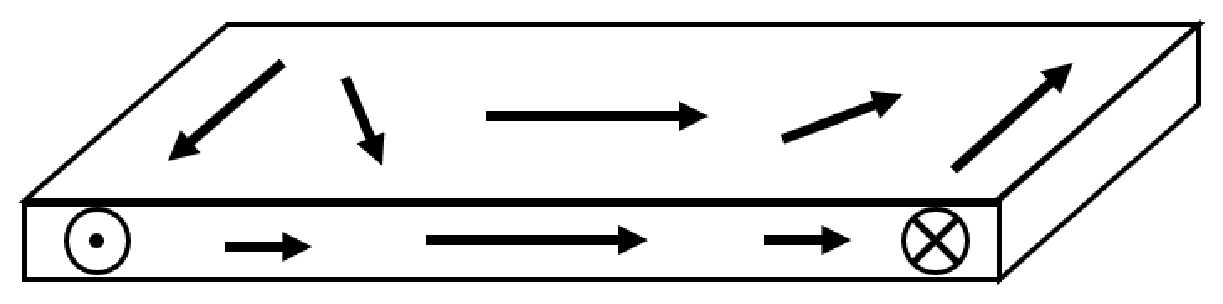
\includegraphics[width=14cm]{pic01.eps}
	\caption{時間と磁壁の前進速度の関係}
	\label{fig01}
\end{figure}

グラフから見て取れるように、解析解で想定されるような一定の速度で磁壁が進んでは行かず、特定の時間から速さが小さくなっていっている。
これは、境界条件が固定境界条件となっているためだ。
そのため、本来の定常状態における磁壁の前進速度に一番近いのは計算開始からおよそ$128\;\mathrm{ns}$秒後になる。

この時点を本レポートでは定常状態と見なすこととする。
また、このときの磁壁の前進速度は$347.5356\;\mathrm{cm/s}$であった。これは解析解で求まる値$397.5434\;\mathrm{cm/s}$と近しい値となっている。
この値の差は、前述のように計算領域の問題で計算を続けられないことによるものだと考えられる。
つまり、計算領域を増やして計算の繰り返し回数を増やすことによって、より解析解の値にシミュレーションの値が近づくのではないかと推測される。

次に問題にある通り、方位角を算出したところ、磁壁の周囲で$\varphi = 2.267$となった。これは解析解で求まる値$\varphi = 2.329$と近しい値だ。
このことから、磁壁の中心以外でも、原子磁気モーメントに外部磁界をかけた際は、この方位角を取りやすいと推測される。

\subsection{小問2}
格子間隔と時間刻みを変化させた場合の効果を調べていく。
まず、時間刻みを大きくしていったところ、$2\;\mathrm{ps}$より大きくしたタイミングで計算が破綻した。

また、同様に格子間隔を広げていったところ、格子間隔を磁壁幅の$1/5$より小さくしたタイミングで計算が破綻したと思われる。
なぜなら、それまではおおよそ$128\;\mathrm{ns}$頃に定常状態になり、そのご速度が落ちていくのに対し、$6\;\mathrm{ns}$ほどで速度が負の値になってしまうからだ。
少なくとも、想定しているような計算結果は得られなかった。

そして、格子間隔を磁壁幅と同程度にしたときは、磁壁の移動が全く見られなかった。

\section{参考文献}

\begin{itemize}
  \item 配布されたテキスト
\end{itemize}

\end{document}